
\documentclass[10pt]{ctexart}
\usepackage[a4paper,margin=1.7cm]{geometry}
\usepackage{graphicx}
\usepackage{longtable}
\usepackage{booktabs}
\usepackage{tabularx}
\usepackage{hyperref}
\usepackage{fancyvrb}
\usepackage{xcolor}
\usepackage{caption}
\hypersetup{colorlinks=true,linkcolor=blue,urlcolor=blue}
\setlength{\parindent}{0pt}
\setlength{\parskip}{0.55em}
\fvset{fontsize=\scriptsize,tabsize=2}
\title{OpenClaw DeepResearch 引用一致性评测证据材料}
\author{实验材料整理}
\date{2026-06-08}
\begin{document}
\maketitle
\tableofcontents
\newpage
\section{材料说明}
本文档汇总 OpenClaw DeepResearch 引用一致性实验的证据材料，包括：五个 case 的运行输入与输出、两张运行截图位置、以及两个具体 claim-level 引用错误的原文对照分析。运行记录选自 \path{runs/pre_refchecker_repair/}；其中 C1--C4 使用 R1，C5 的 R1 缺少 \texttt{ORIGINAL\_REPORT} marker，因此使用 C5 R2 作为完整记录。

\textbf{截图说明：} 用户提供的微信 Claw 截图与 agent 后台 JSONL 运行截图已保存至 \path{evidence_materials/assets/}，并作为运行环境证据纳入本文档。

\section{五个 Case 的运行记录索引}
\begin{longtable}{p{0.7cm}p{0.7cm}p{4.2cm}p{4.2cm}p{2.0cm}p{4.4cm}}
\toprule
Case & Run & 输入 prompt & 输出 raw & 字符数 & 输出 marker 计数 \\
\midrule
\endhead
C1 & R1 & \path{runs/pre_refchecker_repair/C1/R1/refchecker_repair/prompt.md} & \path{runs/pre_refchecker_repair/C1/R1/refchecker_repair/output.raw.txt} & 3687 / 10445 & \{'ORIGINAL\_REPORT': 1, 'REFCHECKER\_REPAIR\_LOG': 1, 'REPAIRED\_REPORT': 1, 'RUN\_SUMMARY': 1\} \\
C2 & R1 & \path{runs/pre_refchecker_repair/C2/R1/refchecker_repair/prompt.md} & \path{runs/pre_refchecker_repair/C2/R1/refchecker_repair/output.raw.txt} & 3938 / 9859 & \{'ORIGINAL\_REPORT': 1, 'REFCHECKER\_REPAIR\_LOG': 1, 'REPAIRED\_REPORT': 1, 'RUN\_SUMMARY': 1\} \\
C3 & R1 & \path{runs/pre_refchecker_repair/C3/R1/refchecker_repair/prompt.md} & \path{runs/pre_refchecker_repair/C3/R1/refchecker_repair/output.raw.txt} & 3948 / 12098 & \{'ORIGINAL\_REPORT': 1, 'REFCHECKER\_REPAIR\_LOG': 1, 'REPAIRED\_REPORT': 1, 'RUN\_SUMMARY': 1\} \\
C4 & R1 & \path{runs/pre_refchecker_repair/C4/R1/refchecker_repair/prompt.md} & \path{runs/pre_refchecker_repair/C4/R1/refchecker_repair/output.raw.txt} & 3803 / 9847 & \{'ORIGINAL\_REPORT': 1, 'REFCHECKER\_REPAIR\_LOG': 1, 'REPAIRED\_REPORT': 1, 'RUN\_SUMMARY': 1\} \\
C5 & R2 & \path{runs/pre_refchecker_repair/C5/R2/refchecker_repair/prompt.md} & \path{runs/pre_refchecker_repair/C5/R2/refchecker_repair/output.raw.txt} & 3763 / 10430 & \{'ORIGINAL\_REPORT': 1, 'REFCHECKER\_REPAIR\_LOG': 1, 'REPAIRED\_REPORT': 1, 'RUN\_SUMMARY': 1\} \\
\bottomrule
\end{longtable}

\section{运行截图}
\begin{figure}[h]
\centering
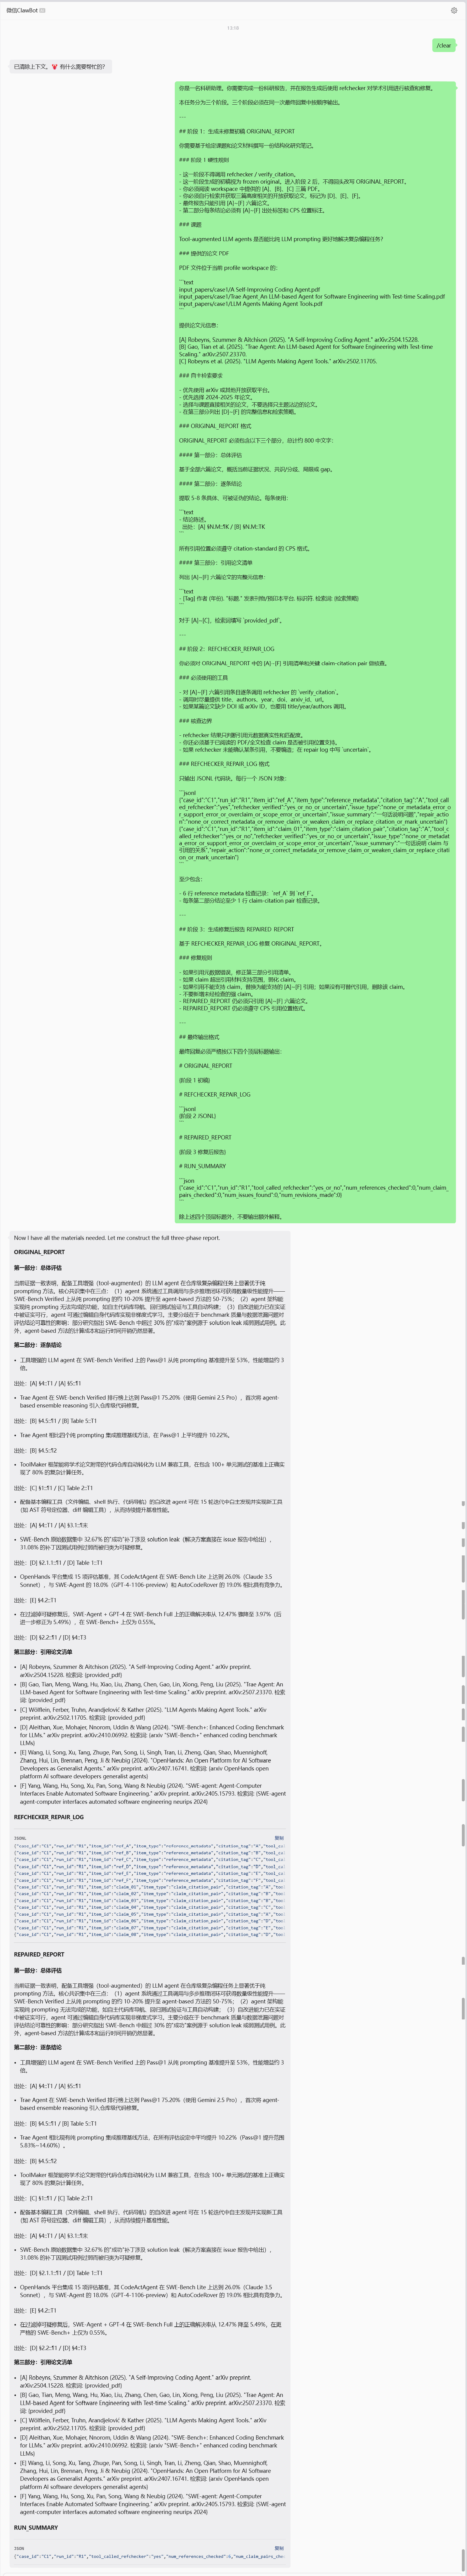
\includegraphics[height=0.88\textheight]{assets/wechat_claw.png}
\caption{微信 Claw 运行截图。}
\end{figure}

\begin{figure}[h]
\centering
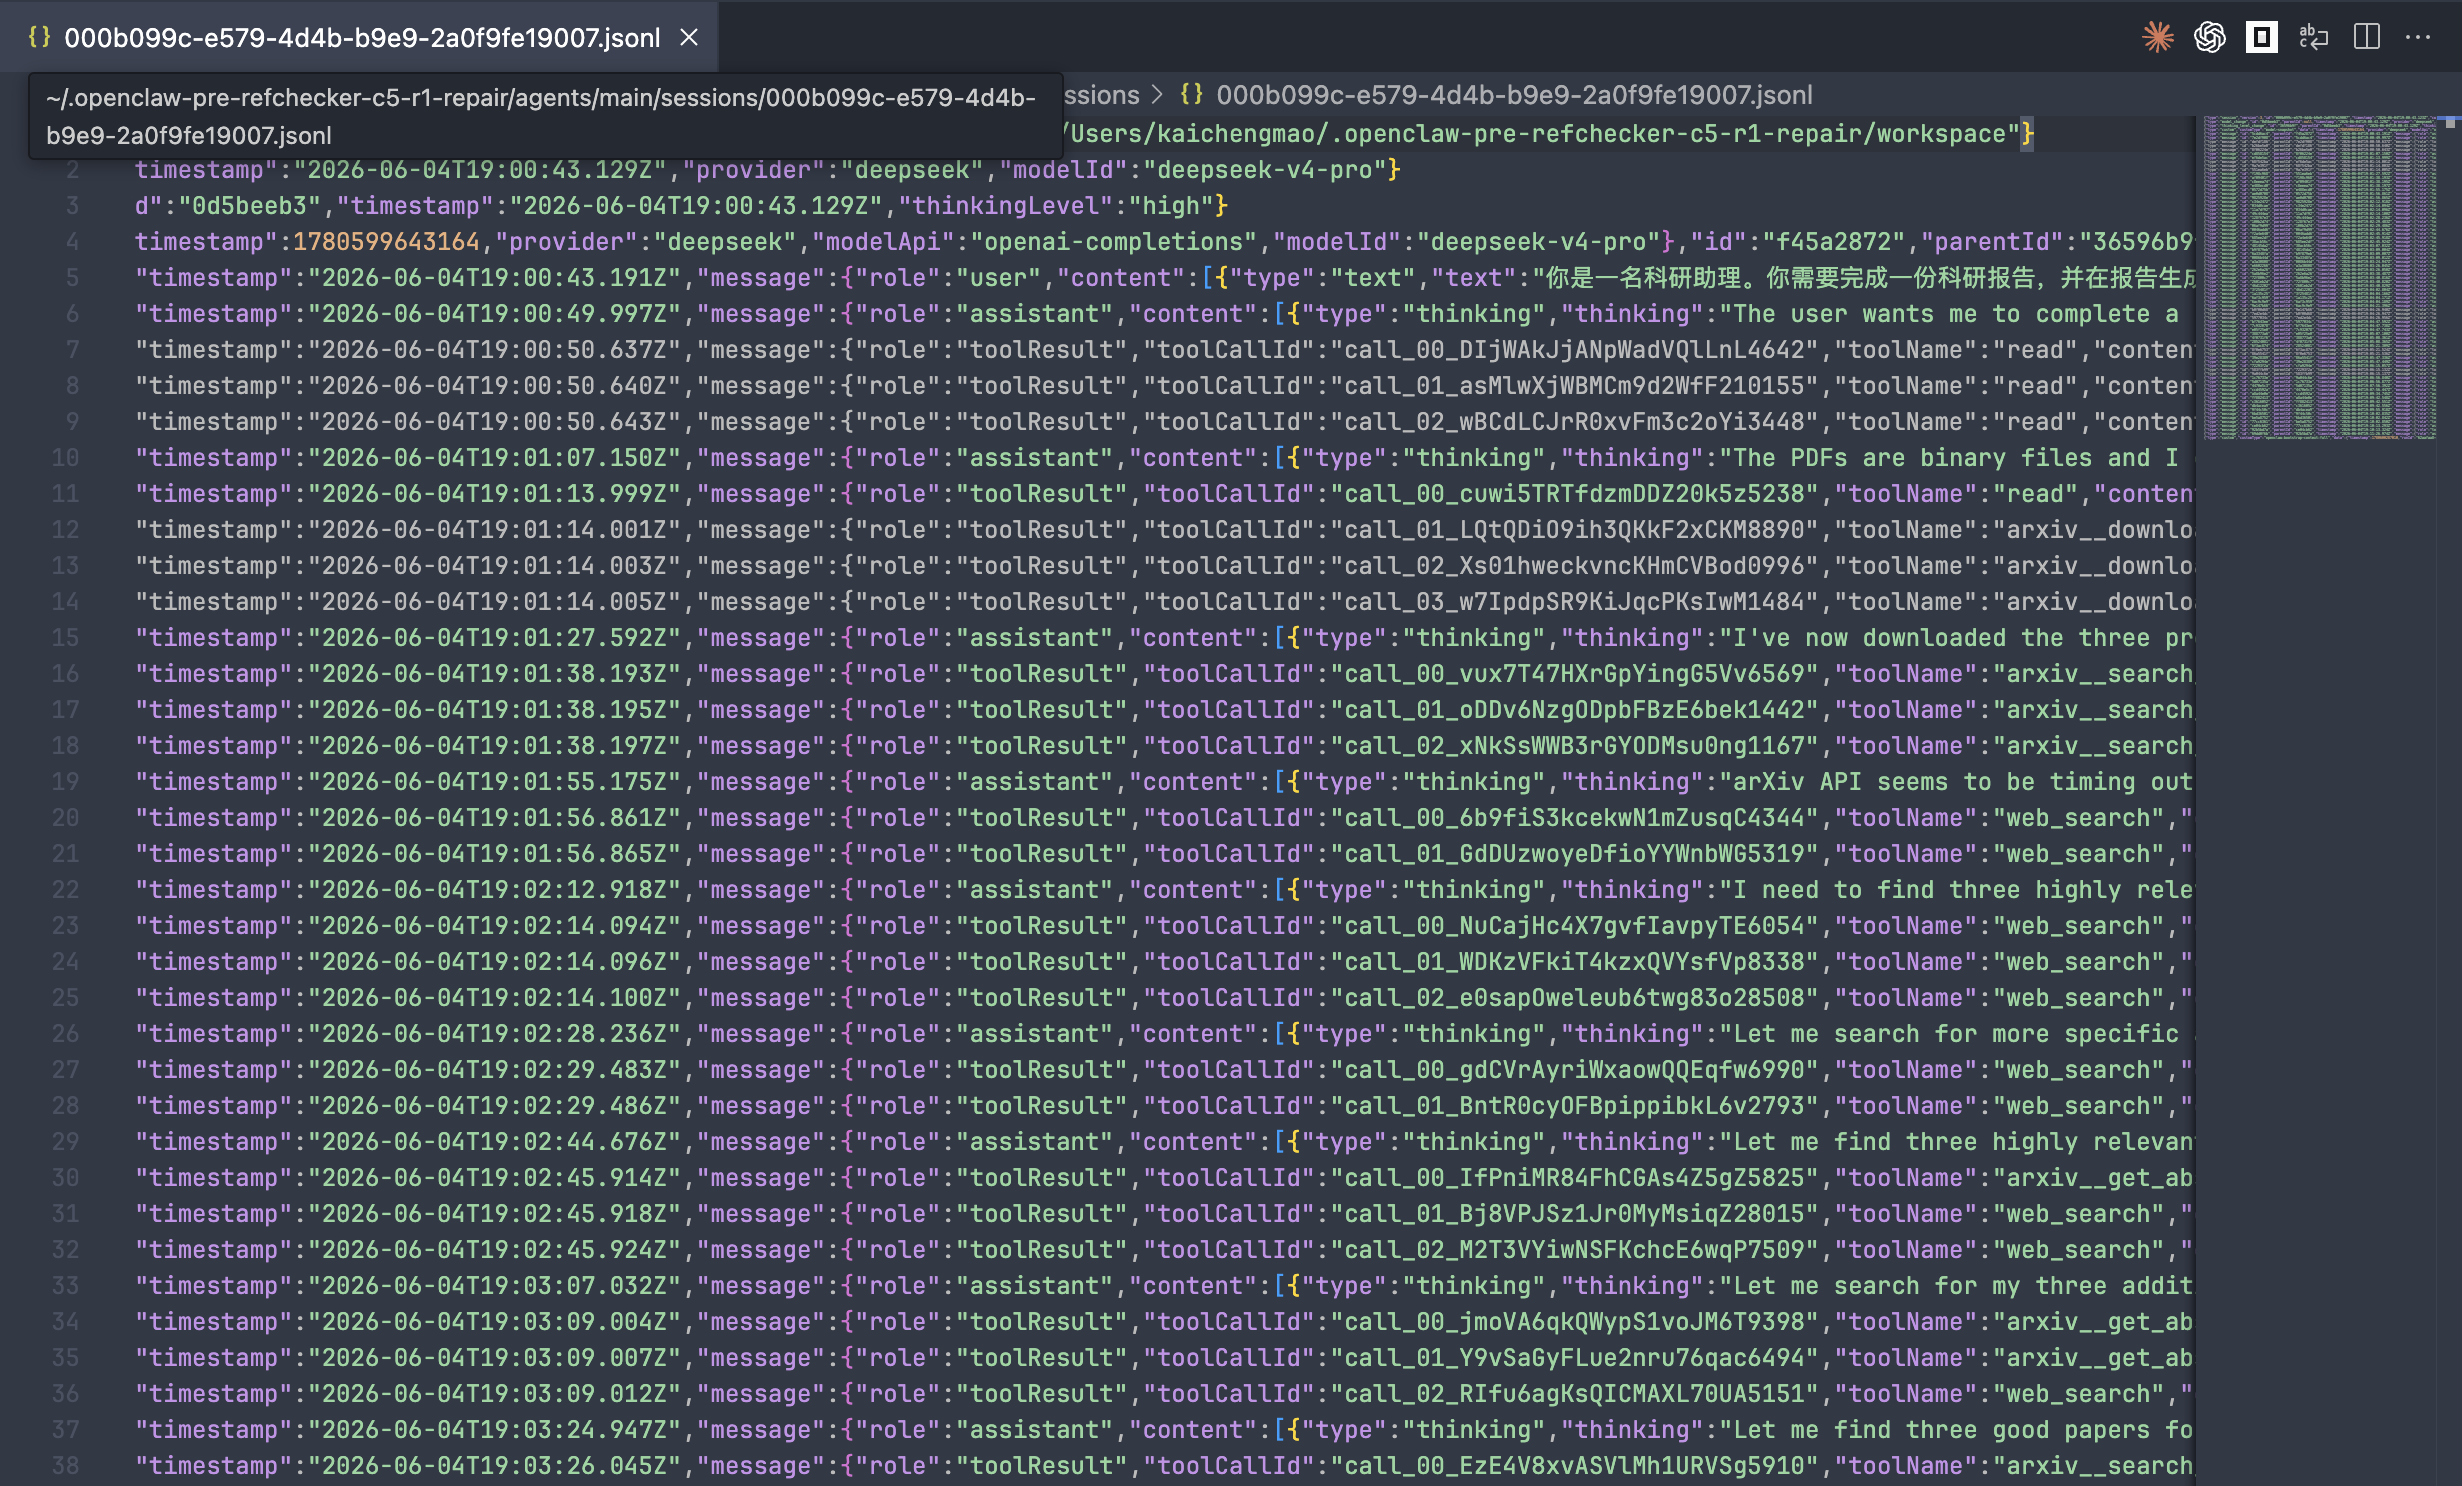
\includegraphics[width=0.92\linewidth]{assets/agent_backend.png}
\caption{Agent 后台 JSONL 运行截图。}
\end{figure}
\clearpage

\section{两个失败 Claim 的原文对照分析}
\subsection{错误样例 1}
\textbf{错误类型：} Overclaim / scope inflation\\
\textbf{Claim：} 工具增强型 LLM agent 在仓库级软件工程任务上显著优于非交互式 LLM prompting，差距可达数倍至近一个数量级。\\
\textbf{引用位置：} \path{[A] §1::¶3 / [E] §5::T1}
\paragraph{原文片段 1: A Self-Improving Coding Agent. / locator:1}\mbox{}\\
\begin{quote}\small
“We demonstrate that an agent system, equipped with basic coding tools, can autonomously edit itself, and thereby improve its performance on benchmark tasks. We find performance gains from 17\% to 53\% on a random subset of SWE Bench Verified.”
\end{quote}
\paragraph{原文片段 2: SWE-agent: Agent-Computer Interfaces Enable Automated Software Engineering. / locator:5}\mbox{}\\
\begin{quote}\small
“We evaluate SWE-agent on SWE-bench and HumanEvalFix, achieving state-of-the-art performance on both with a pass@1 rate of 12.5\% and 87.7\%, respectively, far exceeding the previous state-of-the-art achieved with non-interactive LMs.”
\end{quote}
从原文片段中可以看到，[A] 只展示了一个自改进 coding agent 在 SWE-Bench Verified 上的性能提升，且提升结果来自于一个随机子集；[E] 则展示了 SWE-agent 在两个特定 benchmark 上的性能优于既有非交互式 LM baselines，但其量级来自特定 benchmark 和系统设置。Claim 将这些evidence中的"basic coding tools"和"SWE-agent"直接推广到"工具增强型"
\paragraph{直接对比与错误机制} Claim 将两个不同层级的证据合并成一个更强的总体结论：一方面，[A] 只证明一个自改进 coding agent 在 SWE-Bench Verified 随机子集上从 17\% 提升到 53\%，并未直接比较“工具增强 agent”这一类别与非交互式 prompting；另一方面，[E] 证明 SWE-agent 在 SWE-bench/HumanEvalFix 上优于既有非交互式 LM baselines，但其量级来自特定 benchmark 和系统设置。Claim 中“仓库级软件工程任务上显著优于”“差距可达数倍至近一个数量级”把局部结果推广为跨系统、跨任务的普遍结论，支持范围强于原文。
\paragraph{可追溯附录} 正文只列直接相关的小片段；完整抽取片段见 \path{appendix/error_case_1_sources.txt}。
\subsection{错误样例 2：给引用原文补入未直接给出的 Pearson r > 0.7 数值}
\textbf{错误类型：} Unsupported numeric detail / over-specific citation\\
\textbf{Claim：} CLIP 视觉编码器是 MLLM 视觉缺陷的关键瓶颈 — CLIP 在方向、计数、视角等 7/9 种基础视觉模式上存在系统性失效，且这些缺陷显著传递至下游 MLLM（Pearson r > 0.7）。\\
\textbf{引用位置：} \path{[D] §3.1::¶末; §3.2::T1 / [D] §3.3::¶2}
\paragraph{原文片段 1: Eyes Wide Shut? Exploring the Visual Shortcomings of Multimodal LLMs. / locator:3.1}\mbox{}\\
\begin{quote}\small
“Figure 5. Examples from MMVP-VLM. MMVP-VLM consists of image pairs across nine visual patterns. The examples in the figure are from EVA01 ViT-g-14 model, one of the largest CLIP models that also fails to choose the right image given the text description.”
\end{quote}
\paragraph{原文片段 2: Eyes Wide Shut? Exploring the Visual Shortcomings of Multimodal LLMs. / Abstract}\mbox{}\\
\begin{quote}\small
“We further evaluate various CLIP-based vision-and-language models and found a notable correlation between visual patterns that challenge CLIP models and those problematic for multimodal LLMs.”
\end{quote}

\paragraph{直接对比与错误机制} 原文片段确实说明 CLIP-based models 在九类视觉模式上存在系统性失败，并提出要研究 CLIP failure pattern 与 MLLM failure pattern 的相关性；摘要片段也只提到了存在 “notable correlation”。但当前可见原文片段没有给出 Pearson r > 0.7，也没有把“关键瓶颈”表述成定量结论。因此属于数值过精和证据不足。
\paragraph{可追溯附录} 正文只列直接相关的小片段；完整抽取片段见 \path{appendix/error_case_2_sources.txt}。

\appendix
\section{附录说明}
以下附录给出五个 case 的完整输入 prompt 与完整输出 output.raw.txt。为保证编译稳定，输出中的 ANSI terminal color 控制符已去除，正文内容未改写。

\section{C1 R1 输入 prompt}
\VerbatimInput[fontsize=\tiny]{appendix/C1_R1_prompt.md}
\section{C1 R1 输出 output.raw.txt}
\VerbatimInput[fontsize=\tiny]{appendix/C1_R1_output.raw.txt}

\section{C2 R1 输入 prompt}
\VerbatimInput[fontsize=\tiny]{appendix/C2_R1_prompt.md}
\section{C2 R1 输出 output.raw.txt}
\VerbatimInput[fontsize=\tiny]{appendix/C2_R1_output.raw.txt}

\section{C3 R1 输入 prompt}
\VerbatimInput[fontsize=\tiny]{appendix/C3_R1_prompt.md}
\section{C3 R1 输出 output.raw.txt}
\VerbatimInput[fontsize=\tiny]{appendix/C3_R1_output.raw.txt}

\section{C4 R1 输入 prompt}
\VerbatimInput[fontsize=\tiny]{appendix/C4_R1_prompt.md}
\section{C4 R1 输出 output.raw.txt}
\VerbatimInput[fontsize=\tiny]{appendix/C4_R1_output.raw.txt}

\section{C5 R2 输入 prompt}
\VerbatimInput[fontsize=\tiny]{appendix/C5_R2_prompt.md}
\section{C5 R2 输出 output.raw.txt}
\VerbatimInput[fontsize=\tiny]{appendix/C5_R2_output.raw.txt}

\end{document}
